\chapter{System Architecture}
\label{chp:chap-three}

In this chapter, a overview of the system architecture and the design model of the system is introduced in details. Before introducing all the subsystems part by part, a overview architecture of our system is shown in Fig.\ref{fig:system} Our system is a resource allocation system for allocating WiFi bandwidth capacity to users, and use a pricing mechanism to allocate the bandwidth to every user accordingly. And using the blockchain contract, we target to achieve a robust, transparent and user-friendly system.

\begin{figure}[h]
    \centering
    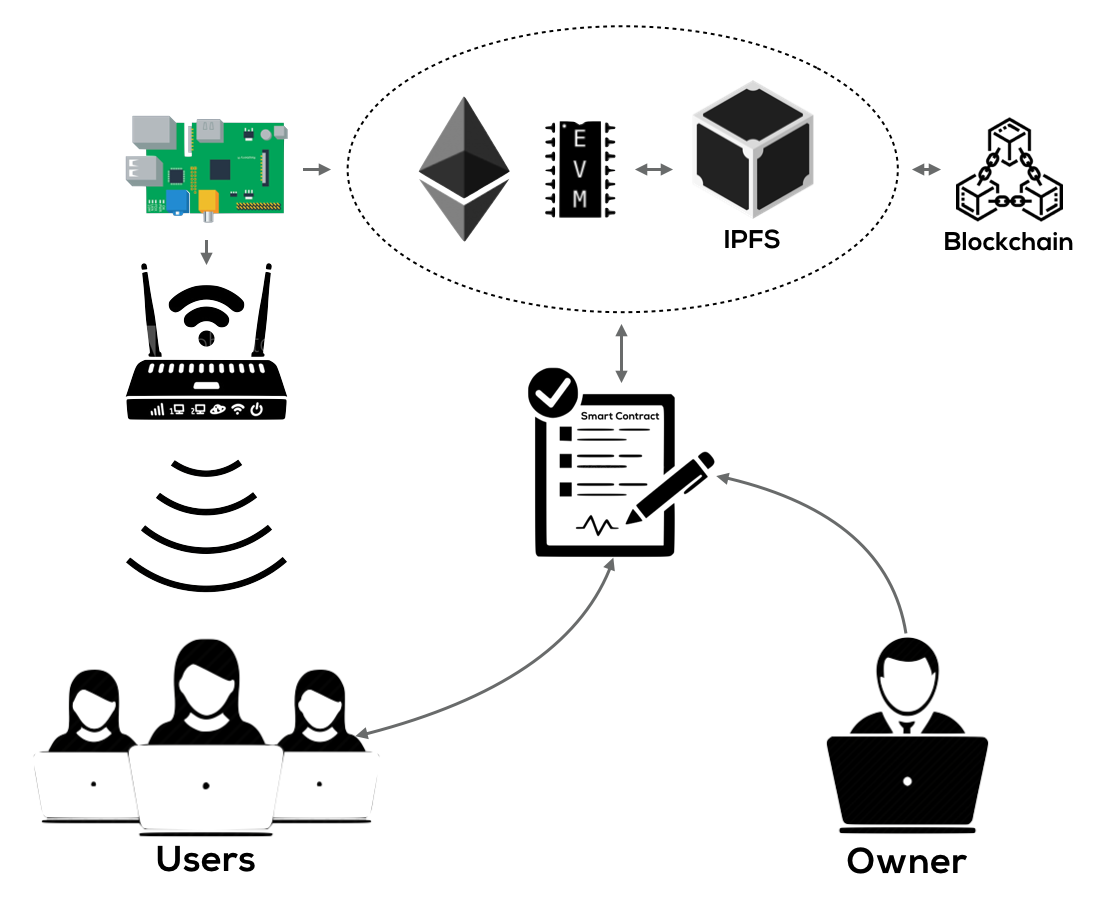
\includegraphics[width=10cm]{My-Thesis/figures/system-architecture.png}    
    \caption{System Architecture}
    \label{fig:system}
\end{figure}

As can be seen from upper Fig.\ref{fig:system}, our system can be mainly divided into two parts -- WiFi Controller and Smart Contract. The two parts currently both are running on the one raspberr pi, whose details would be introduced in Chapter. \ref{chp:chap-five}

\section{WiFi Controller}

\section{Smart Contract}
